\documentclass{beamer}

\usepackage{graphicx}
\usepackage{booktabs}
\usepackage[french]{babel}
%  \usepackage[T1]{fontenc}
%  \usepackage[latin1]{inputenc}
\usepackage{algorithm2e}

\mode<presentation> {
	% \usetheme{default}
	% \usetheme{AnnArbor}
	% \usetheme{Antibes}
	% \usetheme{Bergen}
	% \usetheme{Berkeley}
	% \usetheme{Berlin}
	% \usetheme{Boadilla}
	% \usetheme{CambridgeUS}
	% \usetheme{Copenhagen}
	% \usetheme{Darmstadt}
	% \usetheme{Dresden}
	% \usetheme{Frankfurt}
	% \usetheme{Goettingen}
	% \usetheme{Hannover}
	% \usetheme{Ilmenau}
	% \usetheme{JuanLesPins}
	% \usetheme{Luebeck}
	\usetheme{Madrid}
	% \usetheme{Malmoe}
	% \usetheme{Marburg}
	% \usetheme{Montpellier}
	% \usetheme{PaloAlto}
	% \usetheme{Pittsburgh}
	% \usetheme{Rochester}
	% \usetheme{Singapore}
	% \usetheme{Szeged}
	% \usetheme{Warsaw}

	% \usecolortheme{albatross}
	% \usecolortheme{beaver}
	% \usecolortheme{beetle}
	% \usecolortheme{crane}
	% \usecolortheme{dolphin}
	% \usecolortheme{dove}
	% \usecolortheme{fly}
	% \usecolortheme{lily}
	% \usecolortheme{orchid}
	% \usecolortheme{rose}
	% \usecolortheme{seagull}
	% \usecolortheme{seahorse}
	% \usecolortheme{whale}
	% \usecolortheme{wolverine}

	% \setbeamertemplate{footline} % To remove the footer line in all slides uncomment this line
	% \setbeamertemplate{footline}[page number] % To replace the footer line in all slides with a simple slide count uncomment this line
	\setbeamertemplate{navigation symbols}{} % To remove the navigation symbols from the bottom of all slides uncomment this line
}

\AtBeginSection[]{
	\begin{frame}
		\frametitle{Table des matières}
		\tableofcontents[currentsection]
	\end{frame}
}
\AtBeginSubsection[]{
	\begin{frame}
		\frametitle{Table des matières}
		\tableofcontents[currentsubsection]
	\end{frame}
}

\title[État des lieux]{Plate-forme d'entrainement de gestion de crise}
\author{Brandon Alves, Antoine Boutet}
\institute[INSA Lyon]{
	INSA Lyon \\
	\medskip
	INRIA
}
\date{14 Juin 2021}

\begin{document}
	\begin{frame}
		\titlepage
	\end{frame}
	\begin{frame}
		\frametitle{Table des matières}
		\tableofcontents
	\end{frame}
	\section{Architecture du SI}
		\begin{frame}
			\frametitle{Architecture du SI}
			\begin{block}{Clients}
				\begin{itemize}
					\item debian-client1 (Debian 10)
					\item debian-client2 (Debian 10) : machine du patron
				\end{itemize}
			\end{block}
			\begin{block}{Serveurs}
				\begin{itemize}
					\item debian-web (Debian 9)
					\begin{itemize}
						\item dans DMZ
						\item LAMP
					\end{itemize}
					\item debian-mail (Debian 9)
					\begin{itemize}
						\item Poste.io
					\end{itemize}
					\item debian-dns (Debian 9)
					\begin{itemize}
						\item BIND9
					\end{itemize}
					\item debian-file (Debian 9)
				\end{itemize}
			\end{block}
		\end{frame}
		\begin{frame}
			\frametitle{Architecture du SI}
			\begin{block}{Routeur}
				\begin{itemize}
					\item pfsense (Freebsd)
					\item 5 interfaces (WAN, administration, dmz, clients, services)
					\item Firewall pfSense
					\item DHCP
				\end{itemize}
			\end{block}
			\begin{block}{Attaquant}
				\begin{itemize}
					\item debian-attacker (Debian 9)
					\item dans l'internet
					\item dispose de scripts permettant de lancer différentes attaques
				\end{itemize}
			\end{block}
			\begin{block}{Administrateur}
				\begin{itemize}
					\item debian-admin (Debian 10) : machine de l'administrateur
				\end{itemize}
			\end{block}
		\end{frame}
		\begin{frame}
			\frametitle{Architecture du SI}
			\begin{center}
				\begin{figure}
					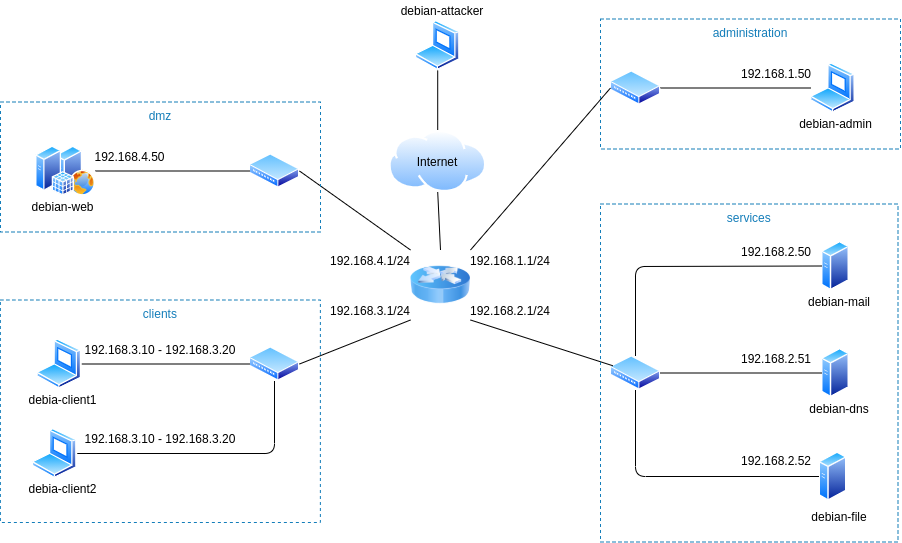
\includegraphics[scale=.3]{si.png}
					\caption{Architecture du SI}
				\end{figure}
			\end{center}
		\end{frame}
	\section{Attaques}
		\begin{frame}
			\frametitle{Attaques}
			\begin{itemize}
				\item Attaque SSH par force brute
				\item Attaque par déni de service (x2 dont \textit{Slowloris})
			\end{itemize}
		\end{frame}
	\section{Informations}
		\begin{frame}
			\frametitle{Comptes utilisateurs}
			\begin{alertblock}{Sur \textit{debian-web}, \textit{debian-dns}, \textit{debian-mail}, \textit{debian-file}, \textit{debian-admin}, \textit{debian-client1} :}
				\begin{description}
					\item[login] admin
					\item[password] password
				\end{description}
			\end{alertblock}
			\begin{alertblock}{Sur \textit{debian-client1} :}
				\begin{columns}
					\begin{column}{.28\linewidth}
						\begin{description}
							\item[login] mcurie
							\item[password] fleur
						\end{description}
					\end{column}
					\begin{column}{.29\linewidth}
						\begin{description}
							\item[login] lpasteur
							\item[password] 12345
						\end{description}
					\end{column}
					\begin{column}{.34\linewidth}
						\begin{description}
							\item[login] hpoincare
							\item[password] motdepasse
						\end{description}
					\end{column}
				\end{columns}
			\end{alertblock}
			\begin{alertblock}{Sur \textit{debian-client2} :}
				\begin{description}
					\item[login] pdupont
					\item[password] argent
				\end{description}
			\end{alertblock}
		\end{frame}
		\begin{frame}
			\frametitle{Mails utilisateurs}
			\begin{alertblock}{admin :}
				\begin{description}
					\item[login] admin@frenchleather.com
					\item[password] password
				\end{description}
			\end{alertblock}
			\begin{alertblock}{pdupont :}
				\begin{description}
					\item[login] pierre.dupont@frenchleather.com
					\item[password] argent
				\end{description}
			\end{alertblock}
		\end{frame}
		\begin{frame}
			\frametitle{Mails utilisateurs}
			\begin{alertblock}{mcurie :}
				\begin{description}
					\item[login] marie.curie@frenchleather.com
					\item[password] fleur
				\end{description}
			\end{alertblock}
			\begin{alertblock}{lpasteur :}
				\begin{description}
					\item[login] louis.pasteur@frenchleather.com
					\item[password] 12345
				\end{description}
			\end{alertblock}
			\begin{alertblock}{hpoincare :}
				\begin{description}
					\item[login] henri.poincare@frenchleather.com
					\item[password] motdepasse
				\end{description}
			\end{alertblock}
		\end{frame}
		\begin{frame}
			\frametitle{SSH}
			Toutes les machines sont accessible par le protocole SSH.
		\end{frame}
		\begin{frame}
			\frametitle{Web}
			Le site internet de l'entreprise est accessible à l'url : \url{www.frenchleather.com}
		\end{frame}
		\begin{frame}
			\frametitle{Messagerie}
			Une interface web de messagerie est disponnible à l'url : \url{mail.frenchleather.com}
		\end{frame}
		\begin{frame}
			\frametitle{NAT}
			\begin{center}
				\begin{figure}
					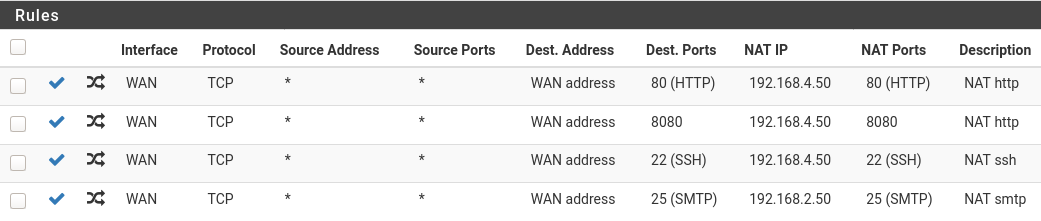
\includegraphics[scale=.3]{nat.png}
					\caption{NAT}
				\end{figure}
			\end{center}
		\end{frame}
	\section{Sujet summer school}
		\begin{frame}
			\frametitle{Sujet summer school}
			\begin{block}{Description}
				\begin{itemize}
					\item FrenchLeather SA
					\item tannerie
					\item région Lyonnaise
					\item travail comporte des risques pour les employés
					\item conditions de travail difficiles
					\item produits toxiques plus aventageux économiquement que produits bios
				\end{itemize}
			\end{block}
		\end{frame}
		\begin{frame}
			\frametitle{Sujet summer school}
			\begin{block}{On peut imaginer \ldots}
				\begin{itemize}
					\item vente en ligne $\rightarrow$ seveur web $\rightarrow$ DoS
					\item adresses de messagerie professionnel $\rightarrow$ piratage du compte du patron $\rightarrow$ chantage
					\item serveur de fichier ? des photos du patron avec sa maitresse ? $\rightarrow$ l'attaquant arrive à s'y introduire récupère les images et fait chanter
					\item serveur de base de données $\rightarrow$ contient : CA, nb de bléssés, salaire, employés non déclarés, \ldots
				\end{itemize}
			\end{block}
		\end{frame}
		\begin{frame}
			\frametitle{Sujet summer school}
			\begin{block}{Autres attaques}
				\begin{itemize}
					\item injection SQL sur le site web de l'entreprise
					\item phishing par mail
					\item ransomeware sur des données sensibles
					\item spyware
				\end{itemize}
			\end{block}
		\end{frame}
	\begin{frame}
		\begin{itemize}
			\item \url{https://www.oodrive.com/fr/blog/securite/top-10-differents-types-cyberattaques/}
			\item \url{https://zeltser.com/malware-sample-sources/}
		\end{itemize}
	\end{frame}
\end{document}
